\documentclass{article}
\usepackage{amsmath}
\usepackage{booktabs}
\usepackage{array}
\usepackage{graphicx}
\usepackage{enumitem}
\usepackage[margin=1in]{geometry}

\title{GATE Petroleum Engineering (PE) 2024}
\date{}

\begin{document}

\maketitle

\section*{General Aptitude (GA)}

\subsection*{Q.1 – Q.5 Carry ONE mark Each}

\begin{table}[h]
\centering
\begin{tabular}{|p{0.9\linewidth}|}
\hline
\textbf{Q.1} If '---' denotes increasing order of intensity, then the meaning of the words [drizzle $\rightarrow$ rain $\rightarrow$ downpour] is analogous to [\_\_\_\_\_ $\rightarrow$ quarrel $\rightarrow$ feud]. Which one of the given options is appropriate to fill the blank? \\
\hline
\begin{tabular}{ll}
(A) & bicker \\
(B) & bog \\
(C) & dither \\
(D) & dodge \\
\end{tabular} \\
\hline
\end{tabular}
\end{table}
\textbf{GATE EE 2025}

\begin{table}[h]
\centering
\begin{tabular}{|p{0.9\linewidth}|}
\hline
\textbf{Q.2} Statements: 1. All heroes are winners. 2. All winners are lucky people. Inferences: I. All lucky people are heroes. II. Some lucky people are heroes. III. Some winners are heroes. Which of the above inferences can be logically deduced from statements 1 and 2? \\
\hline
\begin{tabular}{ll}
(A) & Only I and II \\
(B) & Only II and III \\
(C) & Only I and III \\
(D) & Only III \\
\end{tabular} \\
\hline
\end{tabular}
\end{table}
\textbf{GATE EE 2025}

\begin{table}[h]
\centering
\begin{tabular}{|p{0.9\linewidth}|}
\hline
\textbf{Q.3} A student was supposed to multiply a positive real number $p$ with another positive real number $q$. Instead, the student divided $p$ by $q$. If the percentage error in the student's answer is $80\%$, the value of $q$ is \\
\hline
\begin{tabular}{ll}
(A) & $5$ \\
(B) & $\sqrt{2}$ \\
(C) & $2$ \\
(D) & $\sqrt{5}$ \\
\end{tabular} \\
\hline
\end{tabular}
\end{table}
\textbf{GATE EE 2025}

\begin{table}[h]
\centering
\begin{tabular}{|p{0.9\linewidth}|}
\hline
\textbf{Q.4} If the sum of the first $20$ consecutive positive odd numbers is divided by $20^2$, the result is \\
\hline
\begin{tabular}{ll}
(A) & $1$ \\
(B) & $20$ \\
(C) & $2$ \\
(D) & $1/2$ \\
\end{tabular} \\
\hline
\end{tabular}
\end{table}
\textbf{GATE EE 2025}

\begin{table}[h]
\centering
\begin{tabular}{|p{0.9\linewidth}|}
\hline
\textbf{Q.5} The ratio of the number of girls to boys in class VIII is the same as the ratio of the number of boys to girls in class IX. The total number of students (boys and girls) in classes VIII and IX is $450$ and $360$, respectively. If the number of girls in classes VIII and IX is the same, then the number of girls in each class is \\
\hline
\begin{tabular}{ll}
(A) & $150$ \\
(B) & $200$ \\
(C) & $250$ \\
(D) & $175$ \\
\end{tabular} \\
\hline
\end{tabular}
\end{table}
\textbf{GATE EE 2025}

\section*{Q.6 – Q.10 Carry TWO marks Each}

\begin{table}[h]
\centering
\begin{tabular}{|p{0.9\linewidth}|}
\hline
\textbf{Q.6} In the given text, the blanks are numbered (i)–(iv). Select the best match for all the blanks. \\
Yoko Roi stands \_\_ (i) \_\_ as an author for standing \_\_ (ii) \_\_ as an honorary fellow, after she stood \_\_ (iii) \_\_ her writings that stand \_\_ (iv) \_\_ the freedom of speech. \\
\hline
\begin{tabular}{lllll}
(A) & (i) out & (ii) down & (iii) in & (iv) for \\
(B) & (i) down & (ii) out & (iii) by & (iv) in \\
(C) & (i) down & (ii) out & (iii) for & (iv) in \\
(D) & (i) out & (ii) down & (iii) by & (iv) for \\
\end{tabular} \\
\hline
\end{tabular}
\end{table}
\textbf{GATE EE 2025}

\begin{table}[h]
\centering
\begin{tabular}{|p{0.9\linewidth}|}
\hline
\textbf{Q.7} Seven identical cylindrical chalk-sticks are fitted tightly in a cylindrical container. The figure below shows the arrangement of the chalk-sticks inside the cylinder. The length of the container is equal to the length of the chalk-sticks. The ratio of the occupied space to the empty space of the container is \\
\hline
\begin{tabular}{ll}
(A) & $5/2$ \\
(B) & $7/2$ \\
(C) & $9/2$ \\
(D) & $3$ \\
\end{tabular} \\
\hline
\end{tabular}
\end{table}
\textbf{GATE EE 2025}

\begin{table}[h]
\centering
\begin{tabular}{|p{0.9\linewidth}|}
\hline
\textbf{Q.8} The plot below shows the relationship between the mortality risk of cardiovascular disease and the number of steps a person walks per day. Based on the data, which one of the following options is true? \\
\begin{center}
\includegraphics[width=0.5\textwidth]{risk_plot.png} \\
\end{center}
\hline
\begin{tabular}{p{0.9\linewidth}}
(A) The risk reduction on increasing the steps/day from $0$ to $10000$ is less than the risk reduction on increasing the steps/day from $10000$ to $20000$ \\
(B) The risk reduction on increasing the steps/day from $0$ to $5000$ is less than the risk reduction on increasing the steps/day from $15000$ to $20000$ \\
(C) For any $5000$ increment in steps/day the largest risk reduction occurs on going from $0$ to $5000$ \\
(D) For any $5000$ increment in steps/day the largest risk reduction occurs on going from $15000$ to $20000$ \\
\end{tabular} \\
\hline
\end{tabular}
\end{table}
\textbf{GATE EE 2025}

\begin{table}[h]
\centering
\begin{tabular}{|p{0.9\linewidth}|}
\hline
\textbf{Q.9} Five cubes of identical size and another smaller cube are assembled as shown in Figure A. If viewed from direction X, the planar image of the assembly appears as Figure B. \\
\begin{center}
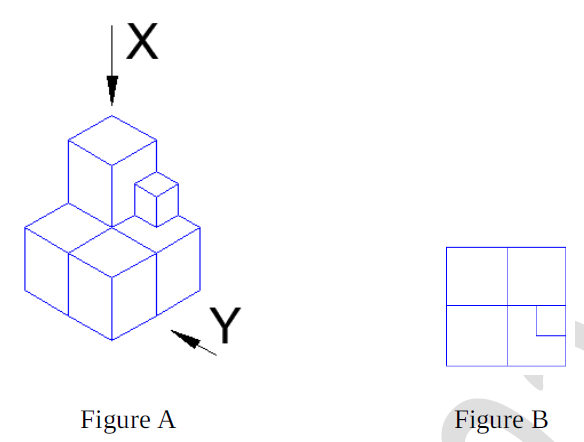
\includegraphics[width=0.5\textwidth]{cubes.png} \\
\end{center}
If viewed from direction Y, the planar image of the assembly (Figure A) will appear as \\
\hline
\begin{tabular}{ll}
(A) & \includegraphics[width=0.2\textwidth]{optionA.png} \\
(B) & \includegraphics[width=0.2\textwidth]{optionB.png} \\
(C) & \includegraphics[width=0.2\textwidth]{optionC.png} \\
(D) & \includegraphics[width=0.2\textwidth]{optionD.png} \\
\end{tabular} \\
\hline
\end{tabular}
\end{table}
\textbf{GATE EE 2025}

\begin{table}[h]
\centering
\begin{tabular}{|p{0.9\linewidth}|}
\hline
\textbf{Q.10} Visualize a cube that is held with one of the four body diagonals aligned to the vertical axis. Rotate the cube about this axis such that its view remains unchanged. The magnitude of the minimum angle of rotation is \\
\hline
\begin{tabular}{ll}
(A) & $120^\circ$ \\
(B) & $60^\circ$ \\
(C) & $90^\circ$ \\
(D) & $180^\circ$ \\
\end{tabular} \\
\hline
\end{tabular}
\end{table}
\textbf{GATE EE 2025}

\section*{Q.11 – Q.35 Carry ONE mark Each}

\begin{table}[h]
\centering
\begin{tabular}{|p{0.9\linewidth}|}
\hline
\textbf{Q.11} A complex number is defined as $z = x + iy$ with $i = \sqrt{-1}$. $\bar{z}$ is the complex conjugate of $z$. The imaginary part of $(2z + 4\bar{z} + 4iy)$ is \_\_\_\_\_\_. \\
\hline
\begin{tabular}{ll}
(A) & $6$ \\
(B) & $2$ \\
(C) & $2y$ \\
(D) & $3y$ \\
\end{tabular} \\
\hline
\end{tabular}
\end{table}
\textbf{GATE EE 2025}

\begin{table}[h]
\centering
\begin{tabular}{|p{0.9\linewidth}|}
\hline
\textbf{Q.12} The solution of the initial value problem given by $y'' + y' - 2y = 0; y(0) = 3, y'(0) = 6$ is \\
\hline
\begin{tabular}{ll}
(A) & $4e^x + e^{-2x}$ \\
(B) & $4e^x - e^{-2x}$ \\
(C) & $4e^x + 3e^{-2x}$ \\
(D) & $4e^{-2x} - 3e^x$ \\
\end{tabular} \\
\hline
\end{tabular}
\end{table}
\textbf{GATE EE 2025}

\begin{table}[h]
\centering
\begin{tabular}{|p{0.9\linewidth}|}
\hline
\textbf{Q.13} The value of the integral $\int_{-\infty}^{\infty} \frac{dx}{1 + x^2}$ is \\
\hline
\begin{tabular}{ll}
(A) & $0$ \\
(B) & $\pi/2$ \\
(C) & $\pi$ \\
(D) & $2\pi$ \\
\end{tabular} \\
\hline
\end{tabular}
\end{table}
\textbf{GATE EE 2025}

\begin{table}[h]
\centering
\begin{tabular}{|p{0.9\linewidth}|}
\hline
\textbf{Q.14} If $A$ is a $3 \times 3$ matrix with eigenvalues $1$, $2$, and $3$, then the determinant of $A^2 - 2A$ is \\
\hline
\begin{tabular}{ll}
(A) & $-6$ \\
(B) & $0$ \\
(C) & $6$ \\
(D) & $24$ \\
\end{tabular} \\
\hline
\end{tabular}
\end{table}
\textbf{GATE EE 2025}

\begin{table}[h]
\centering
\begin{tabular}{|p{0.9\linewidth}|}
\hline
\textbf{Q.15} The probability that a randomly selected bit string of length $10$ contains exactly four $1$'s is \\
\hline
\begin{tabular}{ll}
(A) & $\frac{105}{512}$ \\
(B) & $\frac{63}{256}$ \\
(C) & $\frac{35}{128}$ \\
(D) & $\frac{15}{64}$ \\
\end{tabular} \\
\hline
\end{tabular}
\end{table}
\textbf{GATE EE 2025}

\section*{Q.36 – Q.65 Carry TWO marks Each}

\begin{table}[h]
\centering
\begin{tabular}{|p{0.9\linewidth}|}
\hline
\textbf{Q.36} Which ONE of the following is the implicit form of the solution for the differential equation given below? \\
$\frac{dy}{dx} + \frac{(2x+3y)}{(3x+5y)} = 0$. \\
Note: $C$ in the options below is the integration constant. \\
\hline
\begin{tabular}{ll}
(A) & $x^2 - 3xy - \frac{5y^2}{2} - C = 0$ \\
(B) & $x^2 - 3xy + \frac{5y^2}{2} - C = 0$ \\
(C) & $x^2 + 3xy - \frac{5y^2}{2} - C = 0$ \\
(D) & $x^2 + 3xy + \frac{5y^2}{2} - C = 0$ \\
\end{tabular} \\
\hline
\end{tabular}
\end{table}
\textbf{GATE EE 2025}

\begin{table}[h]
\centering
\begin{tabular}{|p{0.9\linewidth}|}
\hline
\textbf{Q.37} The maximum value of the function $f(x) = x^3 - 6x^2 + 9x + 15$ in the interval $[0, 4]$ is \\
\hline
\begin{tabular}{ll}
(A) & $15$ \\
(B) & $19$ \\
(C) & $23$ \\
(D) & $27$ \\
\end{tabular} \\
\hline
\end{tabular}
\end{table}
\textbf{GATE EE 2025}

\begin{table}[h]
\centering
\begin{tabular}{|p{0.9\linewidth}|}
\hline
\textbf{Q.38} A fair die is rolled twice. Let $X$ be the sum of the two numbers obtained. The variance of $X$ is \\
\hline
\begin{tabular}{ll}
(A) & $\frac{35}{6}$ \\
(B) & $\frac{17}{2}$ \\
(C) & $\frac{35}{12}$ \\
(D) & $\frac{17}{4}$ \\
\end{tabular} \\
\hline
\end{tabular}
\end{table}
\textbf{GATE EE 2025}

\begin{table}[h]
\centering
\begin{tabular}{|p{0.9\linewidth}|}
\hline
\textbf{Q.39} The number of distinct subgroups of the cyclic group $\mathbb{Z}_{12}$ is \\
\hline
\begin{tabular}{ll}
(A) & $4$ \\
(B) & $5$ \\
(C) & $6$ \\
(D) & $7$ \\
\end{tabular} \\
\hline
\end{tabular}
\end{table}
\textbf{GATE EE 2025}

\begin{table}[h]
\centering
\begin{tabular}{|p{0.9\linewidth}|}
\hline
\textbf{Q.40} The solution to the recurrence relation $T(n) = 2T\left(\frac{n}{2}\right) + n\log n$ with $T(1) = 1$ is \\
\hline
\begin{tabular}{ll}
(A) & $O(n)$ \\
(B) & $O(n\log n)$ \\
(C) & $O(n\log^2 n)$ \\
(D) & $O(n^2)$ \\
\end{tabular} \\
\hline
\end{tabular}
\end{table}
\textbf{GATE EE 2025}

\end{document}